\chapter{多目标跟踪算法设计与改进}

\section{多目标跟踪基本任务}
多目标跟踪意为同时对多个目标进行追踪,是计算机视觉中的一项重要技术。多目标跟踪技术在仿真场景中,对于每一帧每一辆行驶的车辆进行多目标跟踪,并为每个被跟踪的目标分配一个唯一的标识符,接着在整个动作序列中能够持续跟踪和识别每个目标。对视频中每个跟踪目标得出他们的坐标数据,获取他们的坐标数据,最后在仿真场景中输出之前被跟踪的每辆车辆的坐标数据完成复现。

本文的主要任务是:

1、收集基于现有仿真场景Town10的交通场景视频,从模拟器中获取目标真实跟踪轨迹的Ground Truth;

2、优化已有的检测跟踪模型,10个性能指标至少3个超过Baseline的5\%;

3、将设计的和现有的模型展示使用可视化方法进行展示。



\section{多目标跟踪的技术挑战}


\subsection{目标外观变化与遮挡}
在诸如yolov5,deepsort等各个算法对多目标跟踪的时候,总是会由于被跟踪的车辆或者行人的姿态,光线光照还有观察视角的变化等原因,这就使得被跟踪的物体基于外观特征的匹配变得困难。与此同时由于是在交通场景下的多目标跟踪,被跟踪的目标与其它不是跟踪目标的物体容易产生遮挡问题。当跟踪目标被遮挡之后,对算法的影响非常之大,常常会导致目标丢失或者是准确性下降。所以在目标外观变化与遮挡这类问题上,是多目标跟踪技术的一个难点。


\subsection{特征数据提取局限性}
在交通场景环境下,提取的跟踪目标特征需要在不同场景、不同条件下具有足够的鲁棒性。但实际情况就是跟踪目标特征(颜色相近、纹理不明显等原因)可能受到各种因素的影响而变得不稳定。在使用多种传感器进行多目标跟踪时,不同的传感器获取的数据会在输出表达结果上存在差异。尤其是在多目标跟踪的跟踪过程中,需要对每个目标分配唯一的一个身份标注,必须确保在整个过程中跟踪目标身份的连续与唯一。所以特征数据提取局限性是多目标跟踪技术的一个难点。

\subsection{实时性与计算效率}
在进行多目标跟踪时,多目标跟踪需要在实时的时间范围之内完成,用来满足多目标跟踪性能或者实际应用的需要。但是跟踪算法的计算复杂度会随着目标数量、传感器数据量以及跟踪算法的复杂性增加而上升。所以,在现用的GPU和CPU等硬件配置的支持下,如何在保证算法跟踪精度的条件下提升算法的计算效率,是多目标跟踪技术的一个难点。



\section{多目标跟踪优化设计理论}
为了优化上文提到的问题,本文在研究中运用了多模态融合和模型优化两项技术理论,在一定程度上解决了传统多目标跟踪在复杂交通场景下不稳定,易断裂的问题,经过仿真实验加实际测试验证证明此算法是可行的,为智慧交通系统的多目标跟踪算法做出优化。如图\ref{fig:np2}是优化流程图,并且以下是详细内容:



\begin{figure}[htbp] % 可以是h(here),t(top),b(bottom),p(page of floats)
	\centering
	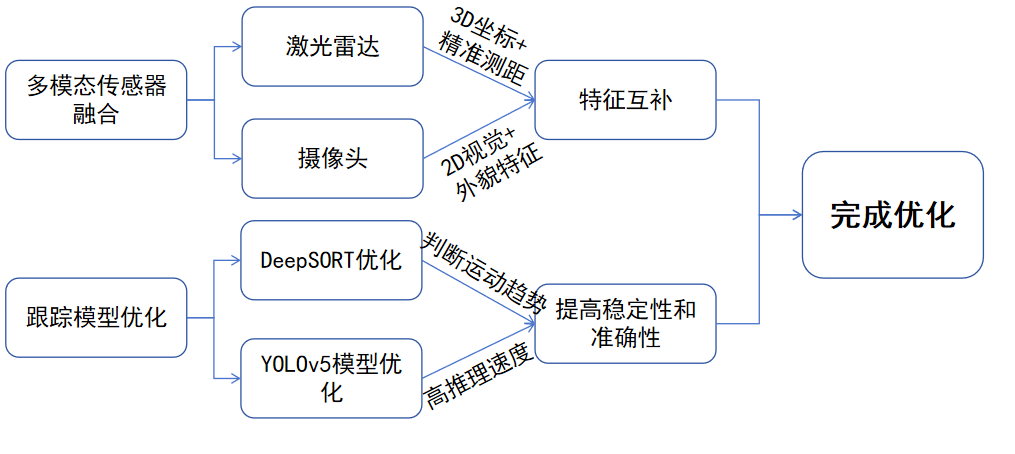
\includegraphics[width=1\textwidth]{np2} % 假设图片文件名为car.pdf或car.png等,位于当前工作目录
	\caption{优化流程图} % 图片标题
	\label{fig:np2} % 用于引用的标签
\end{figure}







采用模型结构与参数优化,面向 Town10 复杂交通环境,对已有检测跟踪模型(YOLOv5、DeepSORT)进行架构改进,借助轻量型网络结构( MobileNet 主干网络)及多尺度融合等方式,在保持实时性的前提下,实现跟踪准确率、稳定性与计算速度等至少 3 项核心指标超越 Baseline5\%以上。

YOLO算法是由主要作者Joseph Redmon在华盛顿大学攻读硕士和博士学位,期间与导师Ali Farhadi共同改进的端到端检测算法。其中YOLOv5算法有如表~\ref{tab:YOLOv5_models}四个版本,本文根据准确性和速度上的需求选择和针对实时性等需求,所以本文选取参数量最少、检测速度最快、识别精度较高的 YOLOv5s 为检测器,并且一定程度上优化YOLOv5s算法。




\begin{table}[htbp]
	\centering
	\caption{YOLOv5 各版本模型对比}
	\label{tab:YOLOv5_models}
	\resizebox{\textwidth}{!}{%
		\begin{tabular*}{\textwidth}{@{\extracolsep{\fill}}lcccccc}
			\toprule
			Model &  mAP (\%) & CPU Speed (ms) & GPU Speed (ms) & Params (M) & FLOPs (B) \\
			\midrule
			yolov5n                             & 45.7              & 45                      & 0.6                     & 1.9                & 4.5               \\
			yolov5s                             & 56.8              & 98                      & 0.9                     & 7.2                & 16.5              \\
			yolov5m                             & 64.1              & 224                     & 1.7                     & 21.2               & 49.0              \\
			yolov5l                             & 67.3              & 430                     & 2.7                     & 46.5               & 109.1             \\
			yolov5x                             & 68.9              & 766                     & 4.8                     & 86.7               & 205.7             \\
			\bottomrule
		\end{tabular*}
	}
\end{table}



DeepSort算法是在Sort算法原有的结构上进行改进开发出来的。



DeepSort是针对Sort在模板跟踪过程中容易发生遮挡导致跟踪目标id切换的问题进行改进。据相关文献\cite{liu2023yolov5deepsort}了解到,DeepSort表现模型为宽残差网络,创新地将外观特征、运动信息两种方法相结合,用结合后的方法进行匹配来解决在模板跟踪过程中遮挡id变化的问题。同时本文了解到DeepSort使用匈牙利分配算法,在跟踪过程中引入表观特征余弦距离度量实现外观特征匹配:\[ d^{(2)}(i,j) = \min \{ 1 - r_j^T r_k^{(i)} \mid r_k^{(i)} \in R_i \} \]其中\(d^{(2)}\)是余弦距离度量结果, \(1 - r_j^T r_k^{(i)}\)用于计算相似性得分,它的阈值需要在训练中找到合适的数值:\[b_{i,j}^{(2)}=\left[d^{(2)}(i,j) \leqslant t^{2}\right]\]马氏距离作用则是短时预判,为降低遮挡引发的 IDS频率,算法通过对余弦距离进行优化改良来完成目标跟踪任务。\[C_{i,j} = \lambda d^{(1)}(i,j) + (1 - \lambda) d^{(2)}(i,j)\]具体流程图如图\ref{fig:np3}。




\begin{figure}[htbp] % 可以是h(here),t(top),b(bottom),p(page of floats)
	\centering
	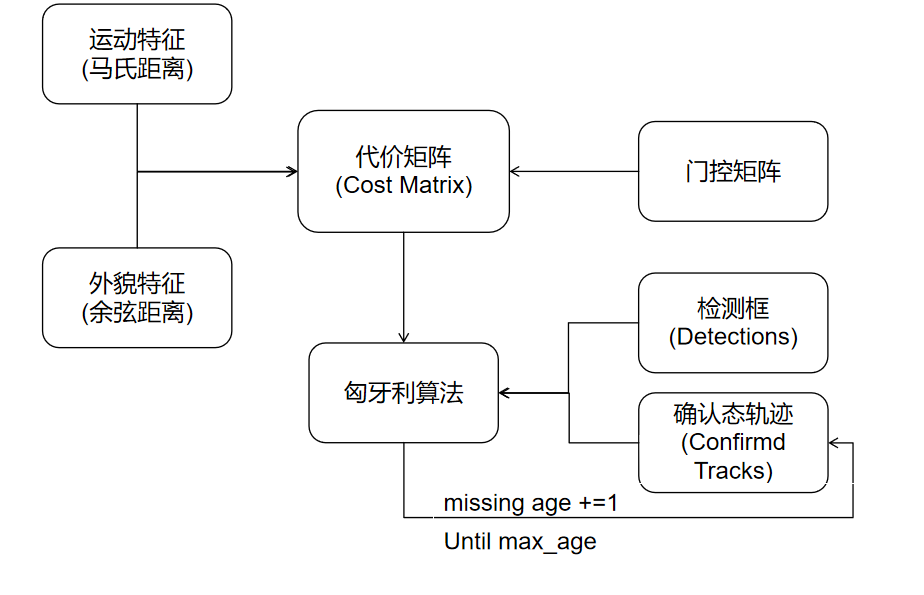
\includegraphics[width=0.75\textwidth]{np3} % 假设图片文件名为car.pdf或car.png等,位于当前工作目录
	\caption{级联匹配流程图} % 图片标题
	\label{fig:np3} % 用于引用的标签
\end{figure}



在DeepSort算法中,针对新生成的轨迹,特别增设了状态确认环节,依据匹配状况将其区分为确认态(Confirmed)与非确认态(Unconfirmed)。新出现的轨迹初始处于非确认态,必须与检测框连续成功匹配三次,方可转变为确认态。若轨迹处于非确认态时,与检测框连续失配次数超出预设的上限值,该轨迹将被系统删除。这种设计有助于提高跟踪的准确性和稳定性,减少误跟踪和轨迹断裂的情况。具体流程图如图\ref{fig:np4}。输入待跟踪视频,若视频结束则流程终止,反之则开始检测。对首帧目标检测框分配 ID,创建初始轨迹并初始化卡尔曼滤波器,初始轨迹为非确认态。更新卡尔曼滤波器,判断轨迹状态。对非确认态轨迹进行IOU匹配,将检测框和预测轨迹匹配结果作为匈牙利算法的代价矩阵,得到最优匹配,轨迹失配则按条件删除或保留轨迹,检测失配则初始化新轨迹并分配新 ID,成功匹配则更新轨迹并预测新位置。轨迹为确认态时进行级联匹配,输出匹配结果并相应处理。循环上述过程直至视频结束。


\begin{figure}[htbp] % 可以是h(here),t(top),b(bottom),p(page of floats)
	\centering
	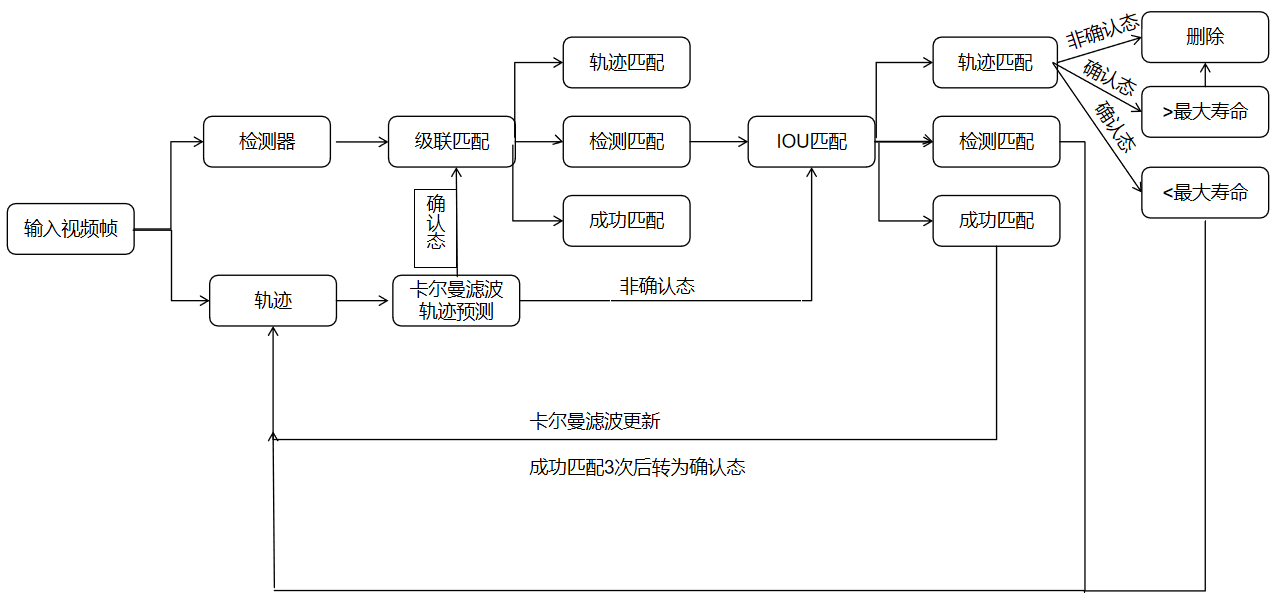
\includegraphics[width=1\textwidth]{np4} % 假设图片文件名为car.pdf或car.png等,位于当前工作目录
	\caption{DeepSort算法流程图} % 图片标题
	\label{fig:np4} % 用于引用的标签
\end{figure}





\subsection{YOLOv5s算法优化}
对于原有的YOLOv5s模型,它本身就是一个目标检测模型,主要侧重于对单帧图像中目标的准确定位和分类,缺乏对目标跨帧关联的能力,在多目标跟踪场景下,难以将检测到的目标在连续帧中进行有效关联,这就容易导致对车辆进行稳定的轨迹跟踪难度较大。并且在复杂交通场景中,当目标被遮挡或与其他目标外观相似时,YOLOv5s很难确定当前帧中检测到的目标与前一帧中的哪个目标对应,容易出现身份切换或轨迹断裂的问题。这一系列问题就产生实时性与精度差、跟踪关联能力有限等问题。因此,本文改进算法的最重要思想就是需要提高算法对多目标连续帧进行有效关联,提高总体的特征提取能力从而提高实时性与精度。


随着visiontransformer的开发与进步\cite{2020arXiv201011929D},本文对YOLOv5s算法的改进是在YOLOv5s算法的主干网络中融入Transformer模块,在融入Transformer模块之后,能够在对小目标检测能力和目标边界模糊检测能力具有提升效果。根据查阅的文献《结合 Swin-Transformer 的改进 YOLOv5s 包装盒缺陷检测算法》\cite{zhao2024jiheswin}帮助下,本文做出如下结构优化图\ref{fig:np5}。

\begin{figure}[htbp] % 可以是h(here),t(top),b(bottom),p(page of floats)
	\centering
	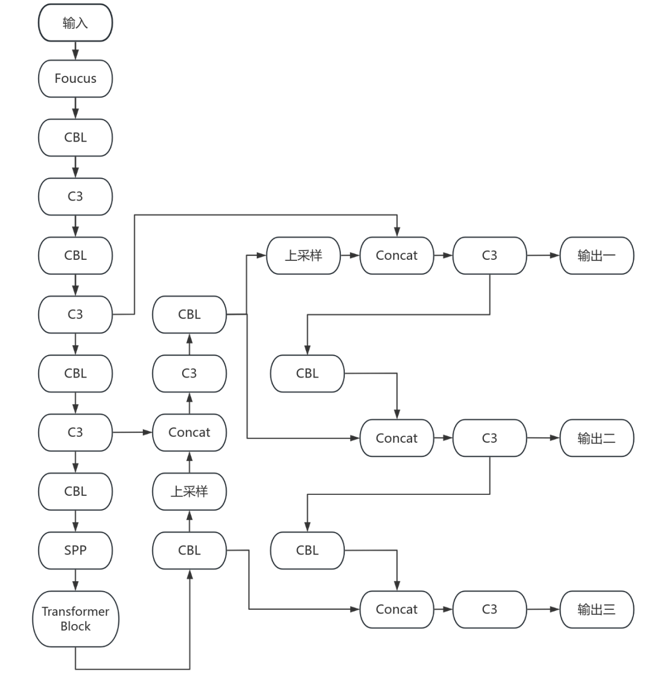
\includegraphics[width=0.5\textwidth]{np5} % 假设图片文件名为car.pdf或car.png等,位于当前工作目录
	\caption{优化后的YOLOv5s结构图} % 图片标题
	\label{fig:np5} % 用于引用的标签
\end{figure}


与传统模块不同,Transformer模块借助特征嵌入和自注意力机制,能够增强特征间的关联性,从而提升全局特征信息的获取效率,进而取得更优的检测效果。同时,Transformer模块还对特征图进行位置信息嵌入以此来确保特征间的有效关联。在改进后的YOLOv5s模型算法中,仅在主干网络的最后部分引入了Transformer模块。实验表明,在网络头部阶段添加Transformer模块可能会因网络深度不够导致语义信息丢失,并且会涉及到边界回归问题。同样是根据上述文献《结合 Swin-Transformer 的改进 YOLOv5s 包装盒缺陷检测算法》了解到的Transformer结构图如图\ref{fig:np6}。

\begin{figure}[htbp] % 可以是h(here),t(top),b(bottom),p(page of floats)
	\centering
	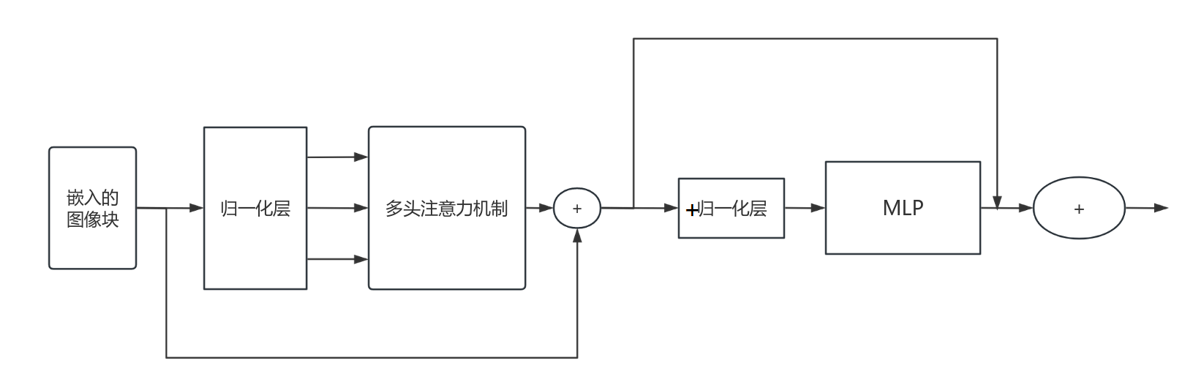
\includegraphics[width=1\textwidth]{np6} % 假设图片文件名为car.pdf或car.png等,位于当前工作目录
	\caption{Transformer结构图} % 图片标题
	\label{fig:np6} % 用于引用的标签
\end{figure}


每个Transformer模块由两个子层构成,第一子层是多头注意力层,第二子层为全连接层(MLP)。Transformer 模块在搜索表征信息时,借助自我注意力机制能够捕捉模型不同位置的信息。



\subsection{DeepSort算法优化}
DeepSort算法能满足本文的需要——“10个性能指标至少3个超过Baseline的5\%”还有所欠缺。本文在实验过程中发现,DeepSort算法虽然能满足基本要求,但是稳定性效果强差人意,在多数实验测试下,能满足要求的寥寥无几,所以本文对DeepSort算法做出了一定优化。


DeepSORT 中用于表观特征提取的原有网络架构相对基础,它仅包含卷两个积层搭配六个残差单元构成的一个简易的 CNN 网络\cite{HLKX202504027}。这样的组合在应对常规且较为简单的场景时,基本能够满足表观特征提取的需求,保障跟踪任务的正常执行。然而,当场景复杂度提升,尤其是存在两个被跟踪目标间相似度极高这种情况时,仅靠这个简单的特征提取网络所获取的信息,作为约束条件就显得力不从心,难以精准地完成跟踪任务。

鉴于这个缺陷,本文在根据已有文献的基础上\cite{DZDK202405010}尝试性地设计了一种新型的特征提取网络架构,经优化升级后的特征提取架构融合了 ECA 结构、RepVGG 网络以及Resnet 网络等模块。此模型着重于增强算法在特征提取方面的能力。其中,结构内的注意力模块与卷积模块采用了轻量化融合策略,对通道数进行了优化改进,有效降低了通道裁剪后可能出现的维度信息缺失问题。旨在显著增强 DeepSort 在表观特征提取的能力方面,使其能够深入且有效地提取图像中蕴含的全局特征以及深层信息,进而实现更加精准、可靠的跟踪效果,有效解决复杂场景下因目标相似度高导致的跟踪难题。其总体结构图如图\ref{fig:np7}所示。以下便是具体算法优化:

\begin{figure}[htbp] % 可以是h(here),t(top),b(bottom),p(page of floats)
	\centering
	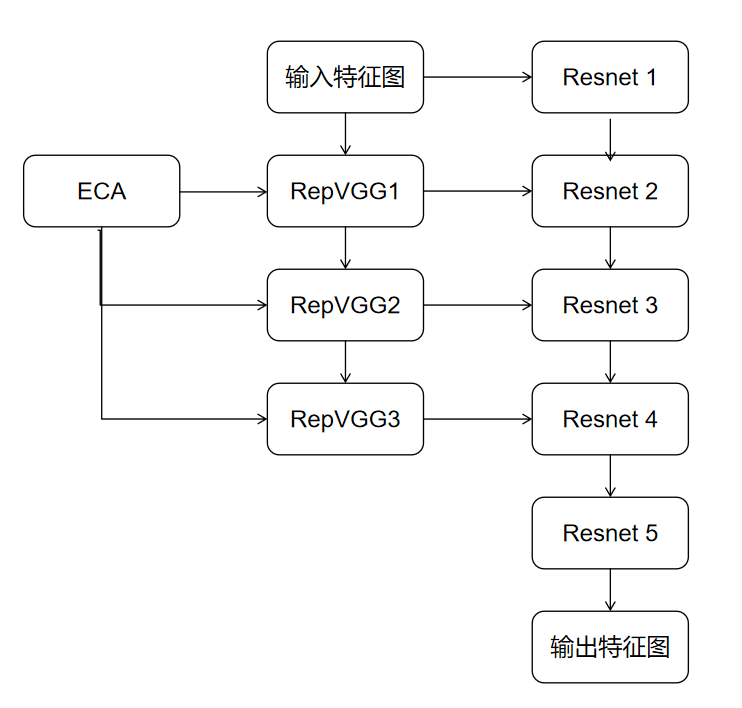
\includegraphics[width=0.5\textwidth]{np7} % 假设图片文件名为car.pdf或car.png等,位于当前工作目录
	\caption{优化结构图} % 图片标题
	\label{fig:np7} % 用于引用的标签
\end{figure}


\subsubsection{ECA注意力机制}

本文将通道注意力模块\cite{QCYK20250429002}引入表观模型,以增强其特征提取效果。在与网络前期的卷积层融合时,优化的网络更聚焦于图像的局部特征,以区分关键信息与次要信息。在深度卷积层中,为优化信道权重以达到最佳性能,多个 ECA 模块被串联,借此可获得最大的注意力区域,进而提高特征提取的准确性与表达力。此外,ECA 通道注意力模块能自适应地调整与分配特征,增强小目标特征图的权重,弥补卷积模块在通道范围内的不足。最终,模型借助 ECA 注意力,使网络能更加专注于被跟踪目标的特征信息,抑制背景干扰,集中注意力于最相关的特征上。在实验中,采用不同尺寸的卷积核将输入特征图分割为多尺度特征图,避免降维,同时有效捕捉跨通道的交互特征。根据上文引用到的文献可了解并作出ECA模块结构图如图\ref{fig:np8}所示。C 是通道数,H 是高度,W 是宽度。图中内容表示对每个通道进行卷积操作之后应用激活函数来引入非线性,增强模型的表达能力然后输出特征图,特征图仍然保持 C×H×W 的维度,但通道之间的信息经过重新调整和加权。

\begin{figure}[htbp] % 可以是h(here),t(top),b(bottom),p(page of floats)
	\centering
	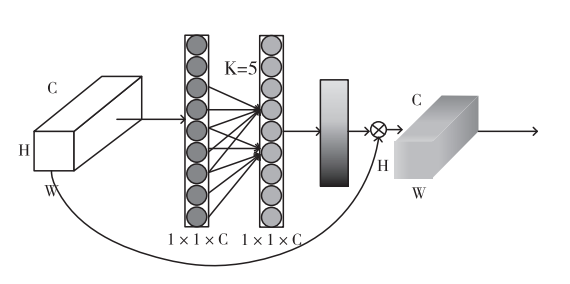
\includegraphics[width=0.8\textwidth]{np8} % 假设图片文件名为car.pdf或car.png等,位于当前工作目录
	\caption{ECA结构图} % 图片标题
	\label{fig:np8} % 用于引用的标签
\end{figure}

\subsubsection{RepVGG网络结构}

本文选用RepVGG\cite{KXJS202307031}这一简单结构的卷积网络引入到DeepSort模型算法中去。在训练阶段,RepVGG模型的块通过多分支结构(包含标准卷积层和可选恒等映射分支)来改善梯度流动、提升训练效率与性能,同时利用参数共享机制,使多个分支在计算资源与参数利用率方面达到高效利用。当它在推理阶段,将训练时的多分支结构重新参数化为一个简单的单分支结构,从而显著降低了推理时的计算复杂度。因为RepVGG算法其每个卷积层仅由基础的卷积操作构成,便于分析各层的特征提取效能,进而通过参数调整达到优化性能的目的。根据文献\cite{KJPL202501006}了解到使用3个RepVGG网络效果比较好,所以本文也是选用3个RepVGG网络来进行特征提取,RepVGG网络训练阶段计算公示为:\[y = \text{ReLU}\left( \text{BN}_{3\times3}(\text{Conv}_{3\times3}(x)) + \text{BN}_{1\times1}(\text{Conv}_{1\times1}(x)) + \text{BN}_{\text{Identity}}(x) \right)\]
其中x为输入,Conv代表卷积操作,BN表示批量归一化层,ReLU为激活函数。
RepVGG网络训练阶段计算公示为:\[y = \text{ReLU}\left( \text{Conv}_{3\times3}^{\text{eq}}(x) \right)\]
其中\(\text{Conv}_{3\times3}^{\text{eq}}\)表示等效的 3×3 卷积操作,该卷积操作是通过对训练阶段的多个分支进行融合得到的。
其结构图如图所示\ref{fig:np16}。


\begin{figure}[htbp] % 可以是h(here),t(top),b(bottom),p(page of floats)
	\centering
	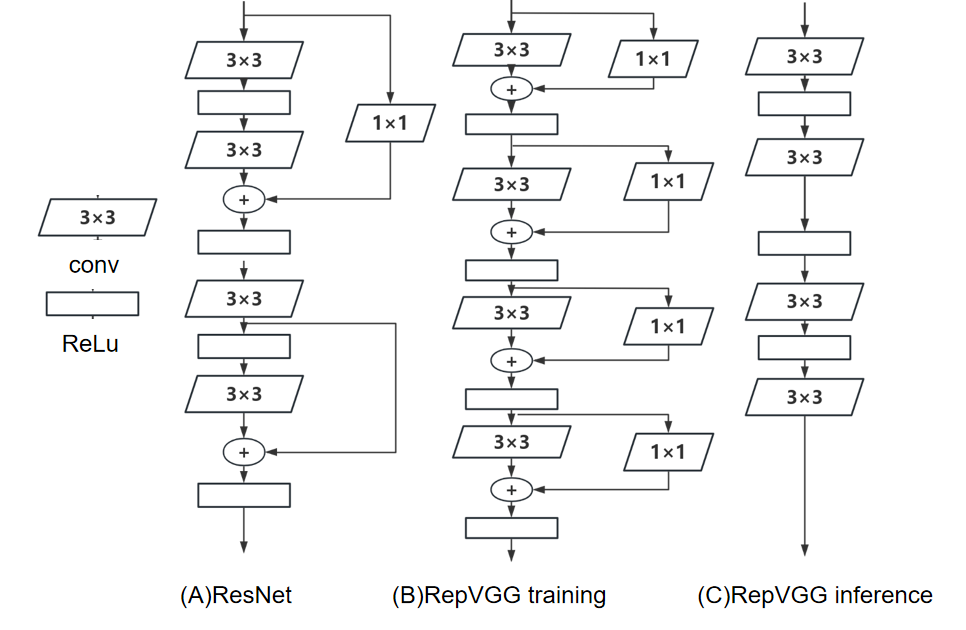
\includegraphics[width=1\textwidth]{np16} % 假设图片文件名为car.pdf或car.png等,位于当前工作目录
	\caption{RepVGG网络结构图} % 图片标题
	\label{fig:np16} % 用于引用的标签
\end{figure}

\subsubsection{RepVGG网络结构}


\section{DeepSort与YOLOv5s架构概述}

本文对多目标跟踪算法优化思路就在于用优化YOLOv5s做检测,用优化DeepSort做多目标跟踪,他们二者衔接关系如图\ref{fig:np15}协调作用如表~\ref{tab:them}。以下是详细内容:


\subsection{目标检测与多目标跟踪流程衔接}

YOLOv5s作为一款高效的目标检测算法,在多目标跟踪系统中扮演着至关重要的角色。其核心任务是对视频流的每一帧图像进行全面而快速的目标识别,精准定位出图像中各类目标物体的类别,并以边界框的形式标定出目标物体在图像中的具体位置。这一过程如同为整个多目标跟踪系统装上了一双敏锐的“眼睛”,使系统能够迅速且精准地捕捉到场景中目标的实时位置,为后续的跟踪任务奠定坚实基础。

DeepSort在YOLOv5s的基础上衔接流程,专注于目标的连续跟踪。它接收来自YOLOv5s提供的目标边界框信息,并结合目标的运动学模型和丰富的外观特征,如颜色、形状等,对不同帧中的目标进行细致的分析和判断,从而精准地确定这些目标是否为同一对象。通过这种方式,DeepSort不仅能够实现对目标的连续跟踪,还能在一定程度上解决目标遮挡、目标消失再出现等复杂场景下的跟踪难题,确保整个多目标跟踪系统在各种动态场景中的稳定性和准确性,为系统的实际应用提供了关键的技术支持。



\subsection{信息交互与融合}
在多目标跟踪系统中,YOLOv5s和DeepSort的协同工作模式发挥了关键作用。首先,YOLOv5s作为目标检测模块,能够快速、准确地提供当前帧中目标的检测框。这些检测框精确框定了目标在图像中的位置范围,为DeepSort进行后续的跟踪操作提供了明确的初始区域,相当于为跟踪任务划定了起始的搜索范围。DeepSort 则在接收到这些检测框后,利用卡尔曼滤波和匈牙利算法等技术,结合目标的运动模型和外观特征,生成平滑且连续的目标运动轨迹。同时,DeepSort对目标外观特征的提取和分析,能够增强模型对目标个体的辨识能力。反过来,这些由DeepSort获得的运动轨迹和外观特征信息,可以作为反馈机制,为YOLOv5s的检测提供参考,帮助检测模块更好地理解目标的运动趋势和外观变化,从而在后续帧中更准确地检测和定位目标,形成一个良性循环,持续提升整个多目标跟踪系统的性能和稳定性。

\subsection{对多目标跟踪性能影响}
YOLOv5s检测器的高效性和准确性对DeepSort算法的性能产生了显著的正面影响。当YOLOv5s能够以极高的精度和速度输出检测结果时,其为DeepSort提供的初始边界框不仅更为精确,而且具有更高的实时性。这种高效准确的输入使得DeepSort能够在更短的时间窗口内接收到更可靠的目标位置信息,从而在目标关联和跟踪过程中占据优势。DeepSort借此可以更迅速地建立和更新目标的状态估计,有效减少误跟踪的情况,同时显著降低ID切换频率,提升整体跟踪的稳定性和准确性。YOLOv5s与DeepSort的这种协同效应,不仅提高了目标跟踪系统的性能,还增强了其在复杂动态场景下的适应性和鲁棒性。


\begin{table}[htbp]
	\centering
	\caption{YOLOv5s 与 DeepSort 协同作用关系}
	\label{tab:them}
	\resizebox{\textwidth}{!}{%
		\begin{tabular}{@{}lll@{}}
			\toprule
			方面               & YOLOv5s                                                                 & DeepSort                                                                                   \\ 
			\midrule
			目标检测与跟踪流程衔接 & \begin{tabular}[c]{@{}l@{}}对每一帧图像进行目标识别,\\ 输出目标类别和边界框位置\end{tabular} & \begin{tabular}[c]{@{}l@{}}接收边界框信息,结合运动状态和外观特征,\\ 判断是否为同一对象,实现连续跟踪\end{tabular} \\ 
			\midrule
			信息交互与融合       & \begin{tabular}[c]{@{}l@{}}提供检测框作为跟踪依据,\\ 明确目标位置范围\end{tabular}          & \begin{tabular}[c]{@{}l@{}}利用目标运动轨迹和外观特征信息,\\ 为检测提供参考\end{tabular}                                                      \\ 
			\midrule
			对多目标跟踪性能影响 & \begin{tabular}[c]{@{}l@{}}高效性和准确性影响输入质量,\\ 精准且迅速的检测结果有助于\end{tabular} & \begin{tabular}[c]{@{}l@{}}获得更准确的初始边界框,\\ 提高跟踪效率,减少误跟踪和 ID 切换\end{tabular}                                       \\ 
			\bottomrule
		\end{tabular}
	}
\end{table}


\begin{figure}[htbp] % 可以是h(here),t(top),b(bottom),p(page of floats)
	\centering
	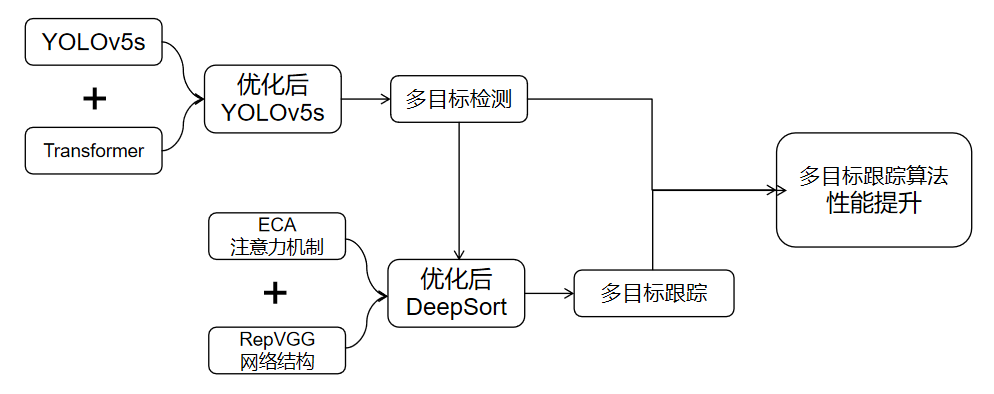
\includegraphics[width=1\textwidth]{np15} % 假设图片文件名为car.pdf或car.png等,位于当前工作目录
	\caption{衔接关系} % 图片标题
	\label{fig:np15} % 用于引用的标签
\end{figure}



\subsection{多模态传感器融合应用}
多模态传感器融合应用,就是将激光雷达与摄像头的相互配合,把他们各自通过观测到的数据结合。本论文提出激光雷达与摄像头数据对象级融合方案,结合激光雷达点云的三维空间坐标及摄像头二维视觉信息以应对复杂交通场景的目标遮挡、断点等问题。用激光雷达的精确的测距能力解决摄像头低照度、复杂的遮挡等问题下的检测盲点, 并以摄像头的外貌特征为对象进行 Re-ID 提供可视信息,完成“探测-跟踪-ReID”的流程,提高多目标跟踪的精准测距能力。

CARLA仿真平台下,多源传感器同步采样及时空同步使得不同数据精确对齐,用于提升目标识别的鲁棒性。
















